\chapter{Casi d'Uso}
\section*{Inizializzazione sistema}

\begin{figure}[ht]
  \centering
  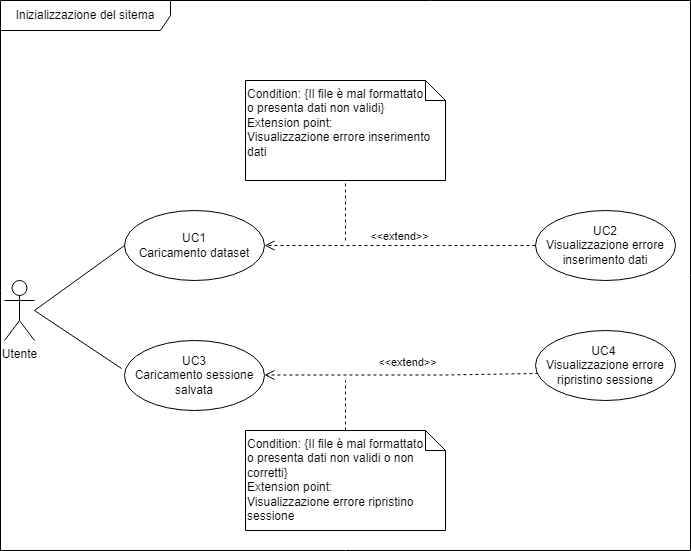
\includegraphics[width=\textwidth]{Iniz_sistema}
  \caption{Inizializzazione del sistema}
\end{figure}
\section{UC1 - Caricamento dataset}
\begin{itemize}
  \item \textbf{Descrizione:} l'utente vuole analizzare un nuovo dataset$_G$ non presente nel sistema;
  \item \textbf{Attore primario:} utente;
  \item \textbf{Precondizioni:} il sistema è raggiungibile e funzionante. L’utente ha a disposizione un dataset in formato CSV$_G$;
  \item \textbf{Postcondizioni:} i dati presenti nel file vengono caricati nel sistema.
  \item \textbf{Scenario principale:}
  \begin{enumerate}
    \item L'utente accede al sistema;
    \item L'utente sceglie un file in formato CSV presente in locale e lo carica nel sistema;
    \item L'utente è pronto ad analizzare i dati.
  \end{enumerate}
  \item \textbf{Estensioni:} nel caso in cui il file sia in un formato non valido o i dati non siano validi:
    \begin{enumerate}
      \item Il caricamento non va a buon fine;
      \item Viene visualizzato un errore esplicativo [UC2].
    \end{enumerate}
\end{itemize}

\section{UC2 - Visualizzazione errore inserimento dati}
\begin{itemize}
  \item \textbf{Descrizione}: l'utente carica un file mal formattato o che presenta dati non validi, quindi visualizza un messaggio di errore esplicativo;
  \item \textbf{Attore Primario:} utente;
  \item \textbf{Precondizioni:} l’utente carica un file CSV contenente i dati da analizzare mal formattato o che presenta dati non validi;
  \item \textbf{Postcondizioni:} l'utente visualizza un messaggio di errore e i dati non vengono caricati;
  \item \textbf{Scenario Principale:}
  \begin{enumerate}
    \item L'utente visualizza un messaggio di errore esplicativo.
  \end{enumerate}
\end{itemize}

\section{UC3 - Caricamento sessione salvata}
\begin{itemize}
  \item \textbf{Descrizione:} l'utente vuole riprendere ad analizzare da dove si era interrotto o ha la necessità di visualizzare una sessione precedente;
  \item \textbf{Attore Primario:} utente;
  \item \textbf{Precondizioni:} l'utente che avvia l'applicativo ha salvato almeno una sessione di lavoro precedente;
  \item \textbf{Postcondizioni:} i dati di una sessione precedentemente salvata vengono ricaricati nel sistema;
  \item \textbf{Scenario Principale:}
  \begin{enumerate}
    \item L'utente accede al sistema;
    \item L'utente sceglie la sessione da caricare selezionando il file JSON$_G$ desiderato tra quelli disponibili,
    cioè tra le sessioni salvate in precedenza;
    \item L'utente riprende da dove aveva salvato.
  \end{enumerate}
  \item \textbf{Estensioni:} nel caso in cui il file JSON selezionato non sia leggibile per qualche possibile errore di salvataggio:
    \begin{enumerate}
      \item Fallisce il caricamento della sessione precedente;
      \item Viene visualizzato un errore esplicativo [UC4].
    \end{enumerate}
\end{itemize}

\section{UC4 - Visualizzazione errore ripristino sessione}
\begin{itemize}
  \item \textbf{Descrizione}: l'utente carica un file mal formattato o che presenta dati non corretti, quindi visualizza un messaggio di errore esplicativo;
  \item \textbf{Attore Primario:} utente;
  \item \textbf{Precondizioni:} l’utente carica un file JSON contenente i dati da analizzare mal formattato o che presenta dati non validi o non corretti;
  \item \textbf{Postcondizioni:} l'utente visualizza un messaggio di errore e i dati non vengono caricati;
  \item \textbf{Scenario Principale:}
  \begin{enumerate}
    \item L'utente visualizza un messaggio di errore esplicativo.
  \end{enumerate}
\end{itemize}

\section{UC5 - Generazione del grafico}
\begin{figure}[H]
 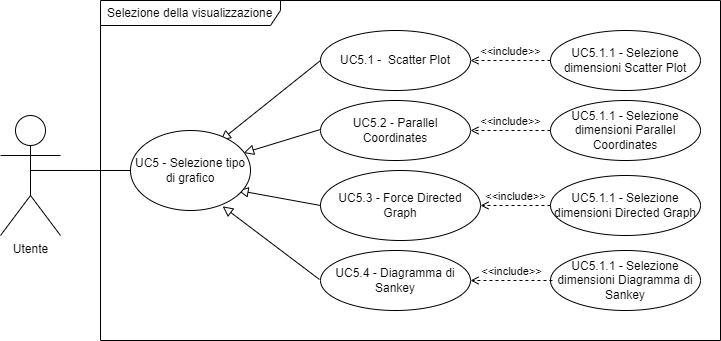
\includegraphics[width=\textwidth]{uc5.png}
 \caption{UC5 - Generazione del grafico}
\end{figure}

 \begin{itemize}
     \item \textbf{Descrizione:} l'utente ha a disposizione varie tipologie di grafico e ne sceglie una;
     \item \textbf{Attore primario:} utente;
     \item \textbf{Precondizioni:} il sistema è stato inizializzato [UC1];
     \item \textbf{Postcondizioni:} è stato selezionato il tipo di grafico da visualizzare;
     \item \textbf{Scenario principale:}
     \begin{enumerate}
       \item L'utente sceglie il tipo di grafico da visualizzare;
     \end{enumerate}
     \item \textbf{Generalizzazioni:} l'utente può selezionare una tra le possibili opzioni:
     \begin{enumerate}
         \item \textit{Scatter Plot}$_G$ [UC5.1];
         \item \textit{Parallel Coordinates}$_G$ [UC5.2];
         \item \textit{Force-Directed Graph}$_G$ [UC5.3];
         \item \textit{Sankey Diagram}$_G$ [UC5.4].
     \end{enumerate}
 \end{itemize}

\subsection{UC5.1 - Generazione Scatter Plot}
\begin{itemize}
    \item \textbf{Descrizione:} l'utente decide la visualizzazione \textit{Scatter Plot};
    \item \textbf{Attore primario:} utente;
    \item \textbf{Precondizioni:} il sistema è stato inizializzato [UC1];
    \item \textbf{Postcondizioni:} è stato selezionato \textit{Scatter Plot} come grafico da visualizzare;
    \item \textbf{Scenario principale:}
    \begin{enumerate}
      \item L'utente sceglie la visualizzazione dei dati mediante \textit{Scatter Plot}.
    \end{enumerate}
\end{itemize}

\subsection{UC5.2 - Generazione Parallel Coordinates}
\begin{itemize}
    \item \textbf{Descrizione:} l'utente decide la visualizzazione \textit{Parallel Coordinates};
    \item \textbf{Attore primario:} utente;
    \item \textbf{Precondizioni:} il sistema è stato inizializzato [UC1];
    \item \textbf{Postcondizioni:} è stato selezionato \textit{Parallel Coordinates} come grafico da visualizzare;
    \item \textbf{Scenario principale:}
    \begin{enumerate}
    \item L'utente sceglie la visualizzazione dei dati mediante \textit{Parallel Coordinates}.
    \end{enumerate}
\end{itemize}

\subsection{UC5.3 - Generazione Force-Directed Graph}
\begin{itemize}
    \item \textbf{Descrizione:} l'utente decide la visualizzazione \textit{Force-Directed Graph};
    \item \textbf{Attore primario:} utente;
    \item \textbf{Precondizioni:} il sistema è stato inizializzato [UC1];
    \item \textbf{Postcondizioni:} è stato selezionato \textit{Force-Directed Graph} come grafico da visualizzare;
    \item \textbf{Scenario principale:}
    \begin{enumerate}
      \item L'utente sceglie la visualizzazione dei dati mediante \textit{Force-Directed Graph}.
    \end{enumerate}
\end{itemize}

\subsection{UC5.4 - Generazione Sankey Diagram}
\begin{itemize}
    \item \textbf{Descrizione:} l'utente decide la visualizzazione \textit{Sankey Diagram};
    \item \textbf{Attore primario:} utente;
    \item \textbf{Precondizioni:} il sistema è stato inizializzato [UC1];
    \item \textbf{Postcondizioni:} è stato selezionato \textit{Sankey Diagram} come grafico da visualizzare;
    \item \textbf{Scenario principale:}
    \begin{enumerate}
      \item L'utente sceglie la visualizzazione dei dati mediante \textit{Sankey Diagram}.
    \end{enumerate}
\end{itemize}

\subsection{UC5.5 - Configurazione Scatter Plot}
\begin{itemize}
    \item \textbf{Descrizione:} l'utente decide la configurazione dello \textit{Scatter Plot};
    \item \textbf{Attore primario:} utente;
    \item \textbf{Precondizioni:} è stato selezionato \textit{Scatter Plot} come grafico da visualizzare [UC5.1];
    \item \textbf{Postcondizioni:} viene visualizzato il grafico \textit{Scatter Plot} con la configurazione scelta;
    \item \textbf{Scenario principale:}
    \begin{enumerate}
      \item L'utente sceglie la configurazione desiderata tra quelle disponibili;
      \item Viene visualizzato il grafico con la configurazione selezionata.
    \end{enumerate}
\end{itemize}

\subsection{UC5.6 - Configurazione Parallel Coordinates}
\begin{itemize}
    \item \textbf{Descrizione:} l'utente decide la configurazione dello \textit{Parallel Coordinates};
    \item \textbf{Attore primario:} utente;
    \item \textbf{Precondizioni:} è stato selezionato \textit{Parallel Coordinates} come grafico da visualizzare [UC5.2];
    \item \textbf{Postcondizioni:} viene visualizzato il grafico \textit{Parallel Coordinates} con la configurazione scelta;
    \item \textbf{Scenario principale:}
    \begin{enumerate}
      \item L'utente sceglie la configurazione desiderata tra quelle disponibili;
      \item Viene visualizzato il grafico con la configurazione selezionata.
    \end{enumerate}
\end{itemize}

\subsection{UC5.7 - Configurazione Force-Directed Graph}
\begin{itemize}
    \item \textbf{Descrizione:} l'utente decide la configurazione dello \textit{Force-Directed Graph};
    \item \textbf{Attore primario:} utente;
    \item \textbf{Precondizioni:} è stato selezionato \textit{Force-Directed Graph} come grafico da visualizzare [UC5.3];
    \item \textbf{Postcondizioni:} viene visualizzato il grafico \textit{Force-Directed Graph} con la configurazione scelta;
    \item \textbf{Scenario principale:}
    \begin{enumerate}
      \item L'utente sceglie la configurazione desiderata tra quelle disponibili;
      \item Viene visualizzato il grafico con la configurazione selezionata.
    \end{enumerate}
\end{itemize}

\subsection{UC5.8 - Configurazione Sankey Diagram}
\begin{itemize}
    \item \textbf{Descrizione:} l'utente decide la configurazione dello \textit{Sankey Diagram};
    \item \textbf{Attore primario:} utente;
    \item \textbf{Precondizioni:} è stato selezionato \textit{Sankey Diagram} come grafico da visualizzare [UC5.4];
    \item \textbf{Postcondizioni:} viene visualizzato il grafico \textit{Sankey Diagram} con la configurazione scelta;
    \item \textbf{Scenario principale:}
    \begin{enumerate}
      \item L'utente sceglie la configurazione desiderata tra quelle disponibili;
      \item Viene visualizzato il grafico con la configurazione selezionata.
    \end{enumerate}
\end{itemize}

\section{UC6 - Personalizzazione visualizzazione}
\begin{figure}[H]
  \centering
  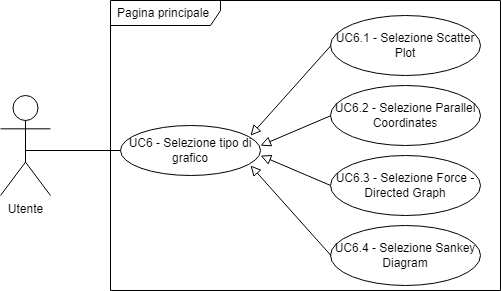
\includegraphics[width=\textwidth]{uc6.png}
  \caption{UC6 - Personalizzazione visualizzazione}
\end{figure}

\begin{itemize}
  \item \textbf{Descrizione}: l'utente ha la possibilità di modificare vari aspetti del grafico;
  \item \textbf{Attore primario}: utente;
  \item \textbf{Precondizioni}: l'utente ha selezionato la tipologia di grafico [UC5] e l'applicativo lo ha generato;
  \item \textbf{Postcondizioni}: le modifiche apportate al grafico vengono visualizzate;
  \item \textbf{Scenario principale}:
   \begin{enumerate}
    \item L'utente può impostare varie opzioni del grafico scelto;
    \item Le opzioni scelte vengono visualizzate.
  \end{enumerate}
  \item \textbf{Generalizzazioni}:
    \begin{enumerate}
      \item Personalizzazione \textit{Scatter Plot} [UC6.1];
      \item Personalizzazione \textit{Parallel Coordinates} [UC6.2];
      \item Personalizzazione \textit{Force-Directed Graph} [UC6.3];
      \item Personalizzazione \textit{Sankey Diagram} [UC6.4].
    \end{enumerate}
\end{itemize}

\subsection{UC6.1 - Personalizzazione Scatter Plot}
\begin{figure}[H]
  \centering
  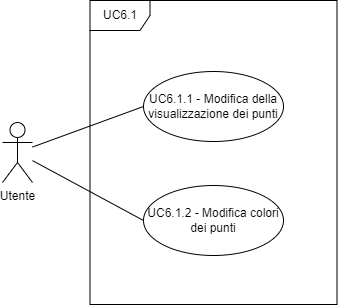
\includegraphics[width=0.6\textwidth]{uc6.1.png}
  \caption{UC6.1 - Personalizzazione Scatter Plot}
\end{figure}
\begin{itemize}
    \item \textbf{Descrizione:} l'utente ha la possibilità di modificare vari aspetti del grafico;
    \item \textbf{Attore primario:} utente;
    \item \textbf{Precondizioni:} l’utente ha scelto il grafico \textit{Scatter Plot} [UC5.1];
    \item \textbf{Postcondizioni:} il grafico viene aggiornato;
    \item \textbf{Scenario principale:}
    \begin{enumerate}
      \item L'utente può decidere di:
    \begin{enumerate}
      \item Modificare visualizzazione dei punti [UC6.1.1];
      \item Modificare colori dei punti  [UC6.1.2].
    \end{enumerate}
    \item Le modifiche scelte vengono visualizzate.
  \end{enumerate}
  \end{itemize}

    \subsubsection{UC6.1.1 - Modifica della visualizzazione dei punti}
  \begin{itemize}
    \item \textbf{Descrizione:} l'utente ha la possibilità di modificare la forma e la dimensione dei punti;
    \item \textbf{Attore primario:} utente;
    \item \textbf{Precondizioni:} l’utente ha scelto il grafico Scatter Plot [UC5.1];
    \item \textbf{Postcondizioni:} il grafico viene aggiornato;
    \item \textbf{Scenario principale:}
     \begin{enumerate}
      \item L'utente sceglie la forma e la dimensione dei punti;
      \item La modifica viene applicata al grafico.
    \end{enumerate}
  \end{itemize}

  \subsubsection{UC6.1.2 - Modifica colori dei punti}
  \begin{itemize}
    \item \textbf{Descrizione:} l'utente ha la possibilità di scegliere i colori dei punti;
    \item \textbf{Attore primario:} utente;
    \item \textbf{Precondizioni:} l’utente ha scelto il grafico Scatter Plot [UC5.1];
    \item \textbf{Postcondizioni:} il grafico viene aggiornato;
    \item \textbf{Scenario principale:}
      \begin{enumerate}
      \item L'utente sceglie i colori dei punti;
      \item La modifica viene applicata al grafico.
    \end{enumerate}
  \end{itemize}

\subsection{UC6.2 - Personalizzazione Parallel Coordinates}
\begin{figure}[H]
 \centering
 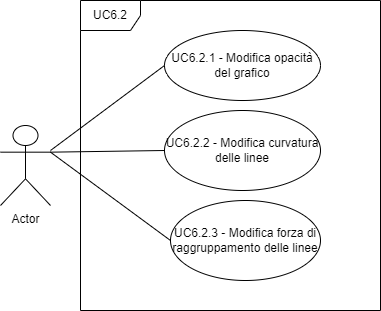
\includegraphics[width=0.6\textwidth]{UC62.png}
 \caption{UC6.2 - Personalizzazione Parallel Coordinates}
\end{figure}
\begin{itemize}
  \item \textbf{Descrizione:} l'utente ha la possibilità di modificare vari aspetti del grafico;
  \item \textbf{Attore primario:} utente;
  \item \textbf{Precondizioni:} l’utente ha scelto il grafico \textit{Parallel Coordinates} [UC5.2];
  \item \textbf{Postcondizioni:} le modifiche apportate al grafico vengono visualizzate;
  \item \textbf{Scenario principale:}
  \begin{enumerate}
    \item L'utente può decidere di:
  \begin{itemize}
    \item Cambiare l'opacità del grafico [UC6.2.1];
    \item Cambiare la curvatura delle linee [UC6.2.2];
    \item Cambiare la forza di raggruppamento delle linee [UC6.2.3].
  \end{itemize}
  \item Le modifiche scelte vengono visualizzate.
\end{enumerate}
\end{itemize}

\subsubsection{UC6.2.1 - Modifica opacità del grafico}
\begin{itemize}
  \item \textbf{Descrizione:} l'utente ha la possibilità di cambiare l'opacità del grafico;
  \item \textbf{Attore primario:} utente;
  \item \textbf{Precondizioni:} l’utente ha scelto il grafico \textit{Parallel Coordinates} [UC5.2];
  \item \textbf{Postcondizioni:} il grafico viene aggiornato;
  \item \textbf{Scenario principale:}
    \begin{enumerate}
    \item L'utente sceglie il grado di opacità;
    \item La modifica viene applicata al grafico.
  \end{enumerate}
\end{itemize}

\subsubsection{UC6.2.2 - Modifica curvatura delle linee}
\begin{itemize}
  \item \textbf{Descrizione:} l'utente ha la possibilità di cambiare la curvatura delle linee;
  \item \textbf{Attore primario:} utente;
  \item \textbf{Precondizioni:} l’utente ha scelto il grafico \textit{Parallel Coordinates} [UC5.2];
  \item \textbf{Postcondizioni:} il grafico viene aggiornato;
  \item \textbf{Scenario principale:}
    \begin{enumerate}
    \item L'utente sceglie se avere delle linee più curve o più rette;
    \item La modifica viene applicata al grafico.
  \end{enumerate}
\end{itemize}

\subsubsection{UC6.2.3 - Modifica forza di raggruppamento delle linee}
\begin{itemize}
  \item \textbf{Descrizione:} l'utente ha la possibilità di cambiare la forza di raggruppamento delle linee;
  \item \textbf{Attore primario:} utente;
  \item \textbf{Precondizioni:} l’utente ha scelto il grafico \textit{Parallel Coordinates} [UC5.2];
  \item \textbf{Postcondizioni:} il grafico viene aggiornato;
  \item \textbf{Scenario principale:}
    \begin{enumerate}
    \item L'utente sceglie quanto deve essere forte il raggruppamento tra le linee del grafico;
    \item La modifica viene applicata al grafico.
  \end{enumerate}
\end{itemize}

\subsection{UC6.3 - Personalizzazione Force-Directed Graph}
\begin{figure}[H]
  \centering
  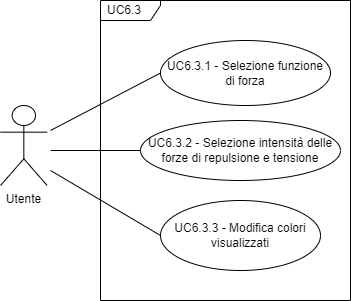
\includegraphics[width=0.6\textwidth]{uc6.3.png}
  \caption{UC6.3 - Personalizzazione Force-Directed Graph}
\end{figure}
\begin{itemize}
    \item \textbf{Descrizione:} l'utente ha la possibilità di modificare vari aspetti del grafico;
    \item \textbf{Attore primario:} utente;
    \item \textbf{Precondizioni:} l’utente ha scelto il grafico \textit{Force-Directed Graph} [UC5.3];
    \item \textbf{Postcondizioni:} il grafico viene aggiornato;
    \item \textbf{Scenario principale:}
    \begin{enumerate}
      \item L'utente può decidere di:
    \begin{enumerate}
      \item Modificare l'intensità della forza di repulsione [UC6.3.1];
      \item Modificare l'intensità della forza di tensione [UC6.3.2];
      \item Modificare i colori visualizzati [UC6.3.3].
    \end{enumerate}
    \item Le modifiche scelte vengono visualizzate.
  \end{enumerate}
  \end{itemize}

  \subsubsection{UC6.3.1 - Modifica intensità della forza di repulsione}
  \begin{itemize}
    \item \textbf{Descrizione:} l'utente ha la possibilità di scegliere quale intensità della forza di repulsione adottare;
    \item \textbf{Attore primario:} utente;
    \item \textbf{Precondizioni:} l’utente ha scelto il grafico Force-Directed Graph [UC5.3];
    \item \textbf{Postcondizioni:} il grafico viene aggiornato;
    \item \textbf{Scenario principale:}
     \begin{enumerate}
      \item L'utente sceglie la funzione di forza;
      \item La modifica viene applicata al grafico.
    \end{enumerate}
  \end{itemize}

  \subsubsection{UC6.3.2 - Modifica intensità della forza di tensione}
  \begin{itemize}
    \item \textbf{Descrizione:} l'utente ha la possibilità di scegliere quale intensità della forza di tensione adottare;
    \item \textbf{Attore primario:} utente;
    \item \textbf{Precondizioni:} l’utente ha scelto il grafico Force-Directed Graph [UC5.3];
    \item \textbf{Postcondizioni:} il grafico viene aggiornato;
    \item \textbf{Scenario principale:}
      \begin{enumerate}
      \item L'utente sceglie l'intensità delle forze;
      \item La modifica viene applicata al grafico.
    \end{enumerate}
  \end{itemize}

  \subsubsection{UC6.3.3 - Modifica colori visualizzati}
  \begin{itemize}
    \item \textbf{Descrizione:} l'utente ha la possibilità di scegliere quali colori adottare;
    \item \textbf{Attore primario:} utente;
    \item \textbf{Precondizioni:} l’utente ha scelto il grafico Force-Directed Graph [UC5.3];
    \item \textbf{Postcondizioni:} il grafico viene aggiornato;
    \item \textbf{Scenario principale:}
     \begin{enumerate}
      \item L'utente sceglie quali colori associare alle varie dimensioni;
      \item La modifica viene applicata al grafico.
    \end{enumerate}
  \end{itemize}

  \subsection{UC6.4 - Personalizzazione Sankey Diagram}
\begin{figure}[H]
  \centering
  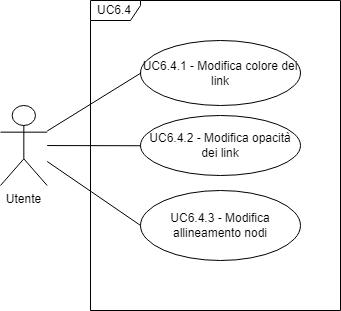
\includegraphics[width=0.6\textwidth]{uc6.4.png}
  \caption{UC6.4 - Personalizzazione Sankey Diagram}
\end{figure}
\begin{itemize}
    \item \textbf{Descrizione:} l'utente ha la possibilità di modificare vari aspetti del grafico;
    \item \textbf{Attore primario:} utente;
    \item \textbf{Precondizioni:} l’utente ha scelto il grafico \textit{Sankey Diagram} [UC5.4];
    \item \textbf{Postcondizioni:} il grafico viene aggiornato;
    \item \textbf{Scenario principale:}
    \begin{enumerate}
      \item L'utente può decidere di:
    \begin{enumerate}
      \item Selezionare il colore dei link [UC6.4.1];
      \item Impostare l'opacità dei link [UC6.4.2];
      \item Selezionare l'allinamento dei nodi [UC6.4.3].
    \end{enumerate}
    \item Le modifiche scelte vengono visualizzate.
  \end{enumerate}
  \end{itemize}

  \subsubsection{UC6.4.1 - Modifica colore dei link}
  \begin{itemize}
    \item \textbf{Descrizione:} l'utente ha la possibilità di scegliere la colorazione dei link, cioè i collegamento tra i nodi;
    \item \textbf{Attore primario:} utente;
    \item \textbf{Precondizioni:} l’utente ha scelto il grafico \textit{Sankey Diagram} [UC5.4];
    \item \textbf{Postcondizioni:} il grafico viene aggiornato;
    \item \textbf{Scenario principale:}
     \begin{enumerate}
      \item L'utente sceglie la colorazione dei link;
      \item La modifica viene applicata al grafico.
    \end{enumerate}
  \end{itemize}

  \subsubsection{UC6.4.2 - Modifica opacità dei link}
  \begin{itemize}
    \item \textbf{Descrizione:} l'utente ha la possibilità di modificare l'opacità dei link;
    \item \textbf{Attore primario:} utente;
    \item \textbf{Precondizioni:} l’utente ha scelto il grafico \textit{Sankey Diagram} [UC5.4];
    \item \textbf{Postcondizioni:} il grafico viene aggiornato;
    \item \textbf{Scenario principale:}
      \begin{enumerate}
      \item L'utente sceglie l'opacità dei link;
      \item La modifica viene applicata al grafico.
    \end{enumerate}
  \end{itemize}

  \subsubsection{UC6.4.3 - Modifica allinamento nodi}
  \begin{itemize}
    \item \textbf{Descrizione:} l'utente ha la possibilità di scegliere l'allineamento dei nodi;
    \item \textbf{Attore primario:} utente;
    \item \textbf{Precondizioni:} l’utente ha scelto il grafico \textit{Sankey Diagram} [UC5.4];
    \item \textbf{Postcondizioni:} il grafico viene aggiornato;
    \item \textbf{Scenario principale:}
     \begin{enumerate}
      \item L'utente sceglie l'allinamento dei nodi;
            \item La modifica viene applicata al grafico.
    \end{enumerate}
  \end{itemize}

\section{UC7 - Filtri sui dati}
\begin{figure}[H]
  \centering
  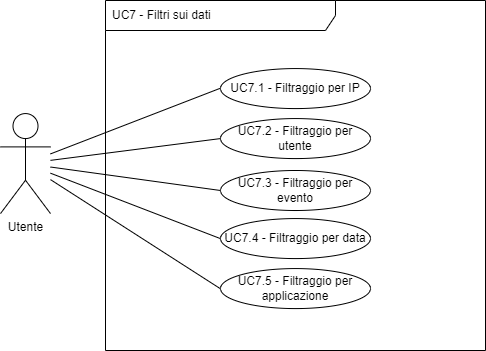
\includegraphics[width=0.8\textwidth]{UC7.png}
  \caption{UC7 - Filtri sui dati}
\end{figure}

\begin{itemize}
  \item \textbf{Descrizione}: l'utente ha la possibilità di modificare la visualizzazione attraverso l'applicazione di filtri sui dati;
  \item \textbf{Attore primario}: utente;
  \item \textbf{Precondizioni}: l'utente ha selezionato la tipologia di grafico [UC5] e l'applicativo lo ha generato;
  \item \textbf{Postcondizioni}: i filtri applicati consentono di mostrare la nuova visualizzazione dei dati sul grafico;
  \item \textbf{Scenario principale}:
    \begin{enumerate}
      \item L'utente può impostare i seguenti filtri tramite una sezione dedicata:
        \begin{itemize}
          \item IP [UC7.1];
          \item Utente [UC7.2];
          \item Evento [UC7.3];
          \item Data [UC7.4];
          \item Applicazione [UC7.5].
        \end{itemize}
      \item Il grafico mostra solo i dati con le caratteristiche corrispondenti alla scelta dei filtri.
    \end{enumerate}
\end{itemize}

\subsection{UC7.1 - Filtraggio per IP}
\begin{itemize}
  \item \textbf{Descrizione}: l'utente ha la possibilità di filtrare i dati in base ad un determinato IP;
  \item \textbf{Attore primario}: utente;
  \item \textbf{Precondizioni}: l'utente ha selezionato la tipologia di grafico [UC5] e l'applicativo lo ha generato;
  \item \textbf{Postcondizioni}: i dati visualizzati sono filtrati in base ad un determinato IP;
  \item \textbf{Scenario principale}:
    \begin{enumerate}
      \item L'utente inserisce l'IP desiderato;
      \item Il grafico mostra solo i dati con l'IP corrispondente.
    \end{enumerate}
\end{itemize}

\subsection{UC7.2 - Filtraggio per utente}
\begin{itemize}
  \item \textbf{Descrizione}: l'utente ha la possibilità di filtrare i dati in base ad un determinato utente;
  \item \textbf{Attore primario}: utente;
  \item \textbf{Precondizioni}: l'utente ha selezionato la tipologia di grafico [UC5] e l'applicativo lo ha generato;
  \item \textbf{Postcondizioni}: i dati visualizzati sono filtrati in base ad un determinato utente;
  \item \textbf{Scenario principale}:
    \begin{enumerate}
      \item L'utente inserisce il numero dell'utente desiderato;
      \item Il grafico mostra solo i dati con il numero dell'utente corrispondente.
    \end{enumerate}
\end{itemize}

\subsection{UC7.3 - Filtraggio per evento}
\begin{itemize}
  \item \textbf{Descrizione}: l'utente ha la possibilità di filtrare i dati in base ad un determinato tipo di evento;
  \item \textbf{Attore primario}: utente;
  \item \textbf{Precondizioni}: l'utente ha selezionato la tipologia di grafico [UC5] e l'applicativo lo ha generato;
  \item \textbf{Postcondizioni}: i dati visualizzati sono filtrati in base ad un determinato tipo di evento;
  \item \textbf{Scenario principale}:
    \begin{enumerate}
      \item L'utente inserisce il tipo di evento desiderato;
      \item Il grafico mostra solo i dati con il tipo di evento corrispondente.
    \end{enumerate}
\end{itemize}

\subsection{UC7.4 - Filtraggio per data}
\begin{itemize}
  \item \textbf{Descrizione}: l'utente ha la possibilità di filtrare i dati in base alla data;
  \item \textbf{Attore primario}: utente;
  \item \textbf{Precondizioni}: l'utente ha selezionato la tipologia di grafico [UC5] e l'applicativo lo ha generato;
  \item \textbf{Postcondizioni}: i dati visualizzati sono filtrati in base alla data;
  \item \textbf{Scenario principale}:
    \begin{enumerate}
      \item L'utente inserisce il periodo temporale desiderato;
      \item Il grafico mostra solo i dati interni al periodo temporale corrispondente.
    \end{enumerate}
\end{itemize}

\subsection{UC7.5 - Filtraggio per applicazione}
\begin{itemize}
  \item \textbf{Descrizione}: l'utente ha la possibilità di filtrare i dati in base ad una determinata applicazione;
  \item \textbf{Attore primario}: utente;
  \item \textbf{Precondizioni}: l'utente ha selezionato la tipologia di grafico [UC5] e l'applicativo lo ha generato;
  \item \textbf{Postcondizioni}: i dati visualizzati sono filtrati in base ad una determinata applicazione;
  \item \textbf{Scenario principale}:
    \begin{enumerate}
      \item L'utente inserisce l'applicazione desiderata;
      \item Il grafico mostra solo i dati relativi all'applicazione corrispondente.
    \end{enumerate}
\end{itemize}


\section{UC8 - Accesso al manuale utente}
\begin{itemize}
  \item \textbf{Descrizione}: l'utente che ha un dubbio o vuole più informazioni sull'utilizzo dell'applicazione, deve avere accesso rapido al manuale utente;
  \item \textbf{Attore primario}: utente;
  \item \textbf{Precondizioni}: nessuna, l'opzione di accesso ai manuali deve essere sempre disponibile all'utente;
  \item \textbf{Postcondizioni}: viene visualizzato il manuale utente;
  \item \textbf{Scenario principale}:
  \begin{enumerate}
    \item L'utente seleziona il manuale utente;
    \item Viene visualizzato il manuale utente.
  \end{enumerate}
\end{itemize}

\section{UC9 - Salvataggio sessione}
\begin{itemize}
  \item \textbf{Descrizione:} l'utente salva la sessione di lavoro;
  \item \textbf{Attore primario:} utente;
  \item \textbf{Precondizioni:} l'utente ha svolto una sessione di lavoro sull'applicazione, in particolare potrebbe aver scelto un grafico specifico e modificato i parametri personalizzando la visualizzazione;
  \item \textbf{Postcondizioni:} l'utente possiede un file JSON in grado di recuperare grafico e parametri impostati durante la sessione di lavoro;
  \item \textbf{Scenario principale:}
  \begin{enumerate}
    \item L'utente sta lavorando sull'applicazione;
    \item L'utente seleziona la funzionalità ``Salvataggio sessione'';
    \item L'utente salva la sessione corrente.
  \end{enumerate}
\end{itemize}
